\documentclass{beamer}
\usetheme{CambridgeUS}
\title{SC2001 Project 2}
\subtitle{The Dijkstra's Algorithm}
\author[Hong, Dinh, He]{Hong Jia Yang \and Dinh Pham Minh Anh \and He Qi Xin}
\institute{Team 4}
\date{\today}

\begin{document}

\begin{frame}
	\titlepage
\end{frame}

\begin{frame}
	\frametitle{Outline}
	\tableofcontents
\end{frame}

\section{Environment Specifications}
\begin{frame}
	\frametitle{Environment}
	\begin{itemize}
		\item Software
		\begin{itemize}
			\item C++
			\item MinGW g++ 13.1.0	
			\item Header \texttt{<bits/std++.h>} 
		\end{itemize}
		\item Hardware
		\begin{itemize}
			\item OS: Windows 11 (Home) x86\_64
			\item Processor: Intel(R) Core(TM) i7-10750H (12) @ 2.59 GHz
		\end{itemize}	
	\end{itemize}
\end{frame}

\section{Implementation of Dijkstra's}
\subsection{Adjacency Matrix and Array}

\begin{frame}
	\frametitle{Matrix Representation of Graph}
	For a graph \( G = (V, E) \), assume that the vertices are numbered \( 1, 2, \hdots, \lvert{ V }\rvert  \) in some arbitrary manner. Then the adjacency-matrix representation of a graph G consists of a \( \lvert{ V }\rvert \times \lvert{ V }\rvert  \) matrix \( A = (a_{ij}) \) such that
	\[
		a_{ij} = \begin{cases}
			w_{ij} & \text{if } (i, j) \in E,\\
			\infty & \text{otherwise.} 
		\end{cases}
	\]

	Where \( w_{ij} \) is the weight for the weight function \( w(u, v) : E \rightarrow \mathbb{R}^+ \) 
	\onslide<2> \begin{block}{Recall}
		Dijkstra's only works for non-negative weighted Directed Graphs	
	\end{block}
\end{frame}

\begin{frame}
	\begin{columns}
	\column{0.5\textwidth}
	\begin{figure}
		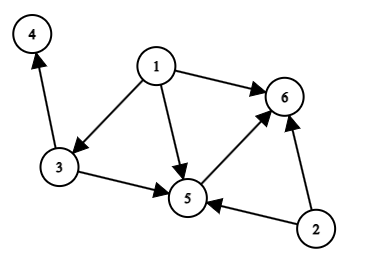
\includegraphics[scale=0.5]{./pict/exampleGraph.png}
		\caption{Graphical Example}
	\end{figure}

	\column{0.5\textwidth}
	\begin{table}
		\begin{tabular}{c|c|c|c|c|c|c}
			  & 1 & 2 & 3 & 4 & 5 & 6\\
			  \hline
			1 & $\infty$ & 1 & $\infty$ & $\infty$ & 1 & 1\\
			\hline
			2 & $\infty$ & $\infty$ & $\infty$ & $\infty$ & 1 & 1\\ 
			\hline
			3 & $\infty$ & $\infty$ & $\infty$ & 1 & 1 & $\infty$ \\
			\hline
			4 & $\infty$ & $\infty$ & $\infty$ & $\infty$ & $\infty$ & $\infty$  \\
			\hline
			5 &  $\infty$ & $\infty$ & $\infty$ & $\infty$ & $\infty$ & 1\\
			\hline
			6 & $\infty$ & $\infty$ & $\infty$ & $\infty$ & $\infty$ & $\infty$\\
			\hline
		\end{tabular}
		\caption{Matrix Representation}
	\end{table}
	\end{columns}
\end{frame}

\begin{frame}
	\frametitle{Implementation of Adjacency Matrix}
	\begin{itemize}
		\item \texttt{std::vector<std::vector<int>>} to represent the 2D array. 
		\begin{itemize}
			\item \texttt{std::vector} is a sequence container that encapsulates dynamic size arrays
			\item 0 indexed
			\item \texttt{INT\_MAX} to represent infinity
		\end{itemize}
		\item Random access: \( O(1) \) 
		\item Insertion or removal of elements at the end: \emph{amortised} \( O(1) \) 
		\item Insertion or removal of elements: \( O(n) \) 
		\item Search whether \( (u,v) \in E \): \( O(1) \) 
		\item Space Complexity: \( O(V^2) \) 
	\end{itemize}
\end{frame}

\subsection{Adjacency List and Minimising Heap}
\begin{frame}
	\frametitle{List Representation of Graph}	
	For a graph \( G = (V, E) \), assume that the vertices are numbered \( 1, 2, \hdots, \lvert{ V }\rvert  \) in some arbitrary manner. Then the adjacency-list representation consists of an array \( Adj \) of \( \lvert{ V }\rvert  \) lists, one for each \( u \in V \). For each \( u \in V\), the adjacency list \( Adj[u] \) is the set
	\[
		Adj[u] = \{ (v, w_{uv}) : (u, v) \in E\}
	\]
	Where \( w_{uv} \) is the weight for the weight function \( w(u, v) : E \rightarrow \mathbb{R}^+ \) 
\end{frame}

\begin{frame}
	\begin{columns}
	\column{0.5\textwidth}
	\begin{figure}
		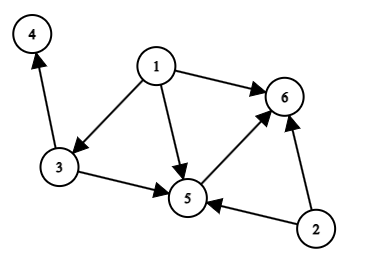
\includegraphics[scale=0.5]{./pict/exampleGraph.png}
		\caption{Graphical Example}
	\end{figure}

	\column{0.5\textwidth}
	\begin{align*}
		1 &: (3, 1) \rightarrow (5, 1) \rightarrow (6, 1)\\
		2 &: (5, 1) \rightarrow (6, 1) \\
		3 &: (4, 1) \rightarrow (5, 1) \\
		4 &: \\
		5 &: (6, 1)\\
		6 &: 
	\end{align*}			
	\centering List Representation
			
	\end{columns}
\end{frame}

\begin{frame}
	\frametitle{Implementation of Adjacency List}
	\begin{itemize}
		\item \texttt{std::vector<std::vector<std::pair<int, int>>>} to represent the adjacency list
		\begin{itemize}
			\item A pair is a specific case of a \texttt{std::tuple} with two elements.
			\item \texttt{vector[u]} is the list for \( u \in V \) 
			\item \texttt{vector[u][i].first} is the index of \( v_i \in V, (u, v_i) \in E \) 
			\item \texttt{vector[u][i].second} is the weight \( w(u, v_i) \) 	
			\item 0 indexed
		\end{itemize}
		\item Search whether \( (u, v) \in E \): \( O(E) \)  
		\item Space Complexity: \( O(V+E) \) 
	\end{itemize}
\end{frame}

\section{Complexity Analysis and Comparison}
\begin{frame}
	
\end{frame}

\end{document}
